\setcounter{section}{8}
\setcounter{subsection}{2}
\setcounter{equation}{13}

	Wir lösen die Schrödingergleichung mit \textbf{Testfunktionen} $\psi_{k}$ und dem \textbf{Variationsprinzip}. 

\paragraph{Variationsprinzip}
	Das Variationsprinzip ist
	$$
	E(k) \ge \frac{\big<\psi_{k}  | \hat{H}  | \psi_{k} \big>}{\left<\psi_{k}  \middle| \psi_{k} \right>}.
	$$

\paragraph{Testfunktionen}
	Als Ansatz wählen wir die lineare Superposition von Atomeigenfunktionen (LCAO) $\varphi_{i} (\Vec{r}-\Vec{r}_{n})$.
	Der Wellenansatz lautet also
	$$
	\begin{aligned}
		\psi_{k} &= \sum_{n}^{} a_{n} \varphi_{i} (\Vec{r}-\Vec{r}_{n})\\
		&= \frac{1}{\sqrt{N} } \sum_{n}^{} e^{i\Vec{k}\Vec{r}_{n}} \varphi_{i} (\Vec{r}-\Vec{r}_{n}).
	\end{aligned}
	$$
	Der Faktor $e^{i\Vec{k}\Vec{r}_{n}}$ in der Summe folgt aus der Forderung, dass $\psi_{k}$ eine \textbf{Blochwelle} ist.
	
\paragraph{Ergebnis} 
	Für kugelsymmetrische, s-artige Atomzustände findet man für die Gesamtenergie
	$$
	E(\Vec{k}) = E_{i} - A - B \sum_{m }^{} e^{i\Vec{k}(r_{n} - r_{m})} ,
	$$ 
	wobei der Index $m$ für eine Summation über die nächsten Nachbarn steht.
	\begin{verbal}
		Die Herleitung ist in \textit{Festkörperphysik} von Gross und Marx zu finden.
	\end{verbal}
	$A$ und $B$ stehen für 
	$$
	\begin{aligned}
		A &= \hspace{8pt}\text{Coulomb-Integral} &&= - \int \text{d}\Vec{r} \varphi_{i} ^{*} (\Vec{r}-\Vec{r}_{n}) V(\Vec{r}-\Vec{r}_{n}) \varphi_{i} (\Vec{r}-\Vec{r}_{n}) \\
		B &= \begin{array}{c} \text{Austausch-Integral} \\ \text{Transfer-Integral}\\ \end{array} \hspace{-9pt}  &&= - \int \text{d}\Vec{r} \varphi_{i}^{*} (\Vec{r}-\Vec{r}_{m})V(\Vec{r}-\Vec{r}_{n}) \varphi_{i}(\Vec{r}-\Vec{r}_{n}).
	\end{aligned}
	$$
	Speziell: für ein \textbf{primitiv kubisches} Gitter mit sechs nächsten Nachbarn pro Atom ist
	$$
	\Vec{r}_{n} - \Vec{r}_{m} = (\pm a, 0, 0);\, (0, \pm a, 0);\, (0, 0, \pm a).
	$$
	Dann beschreibt
	\begin{important}
		$$
		E(\Vec{k}) = E_{i} - A - 2B \left( \cos\left( k_{x} a \right) + \cos\left( k_{y}a \right) + \cos\left( k_{z}a \right)  \right) 
		$$  
	\end{important}
	das elektronische Band, dessen Schwerpunkt um $A$ gegenüber $E_{i}$ abgesenkt ist und dessen Breite $12B$ ist.

\paragraph{Bemerkung}
	Im Festkörper gelten periodische Randbedingungen.
	Jede primitive Elementarzelle trägt genau einen unabhängigen Wert von $k$ zu jedem Energieband bei.
	Bei $N$ Elementarzellen existieren also $N$ Zustände mit jeweils 2 unabhängigen Spinstellungen.
	Insgesamt existieren also $2N$ unabhängige Zustände in jedem Band (bei s-Zuständen; bei p-Zuständen wären es $6N$ Zustände).
	\begin{important}
		Ein volles Band trägt zur Leitfähigkeit nicht bei, da alle Zustände besetzt sind.
	\end{important}

\paragraph{Beispiel} Primitive Elementarzelle: 
	\begin{enumerate}
		\item Einwertiges Atom: 1 Elektron pro Atom $\to $ Das Band ist halbvoll.
		\item Zweiwertiges Atom: 2 Elektronen pro Atom $\to $ Das Band ist voll.
		\item Zwei einwertige Atome: $2 \times 1$ Elektron pro Atom $\to $ Das Band ist voll 
	\end{enumerate}

	\begin{figure}[H]
		\centering
		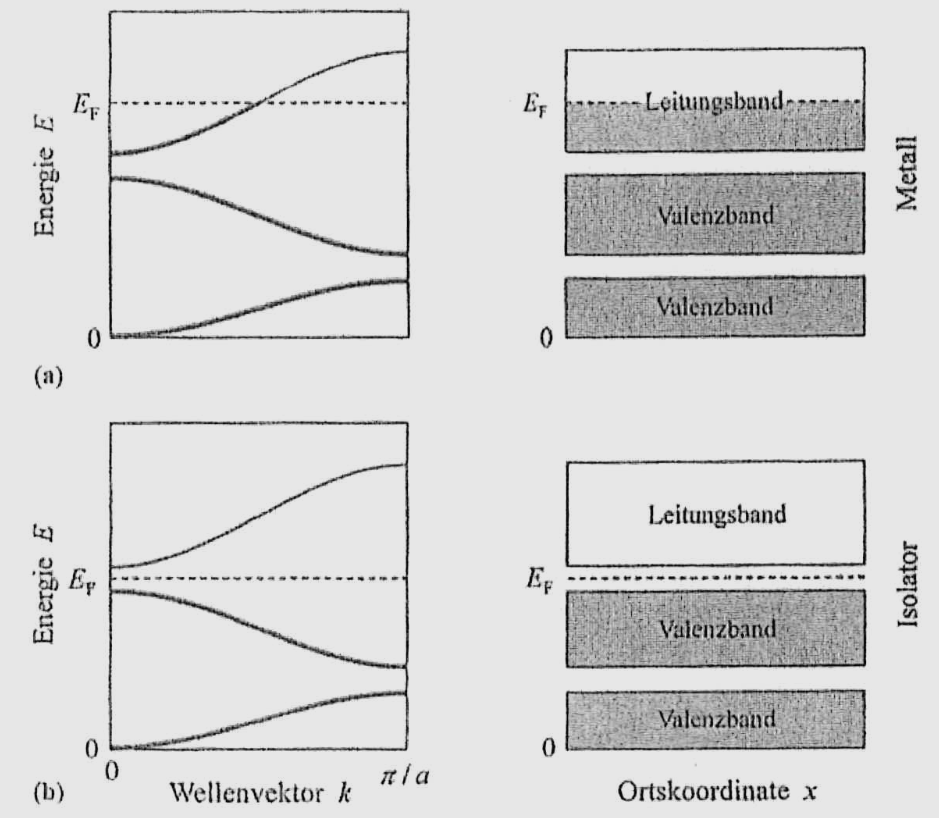
\includegraphics[width = 0.7\linewidth]{figures/vl28/baender_einatomige_basis.png}
		\caption{Dispersionsrelation und Bänderbesetzung zweier Kristalle mit einatomiger Basis \cite{Hunklinger}. 
			Die oberen Bandstrukturen zeigen ein Metall mit vollen Valenzbändern und halbvollem Leitungsband.
			Unten ist ein Isolator zu sehen mit vollen Valenzbändern und leerem Leitungsband.
		}
	\end{figure}
	\begin{figure}[H]
		\centering
		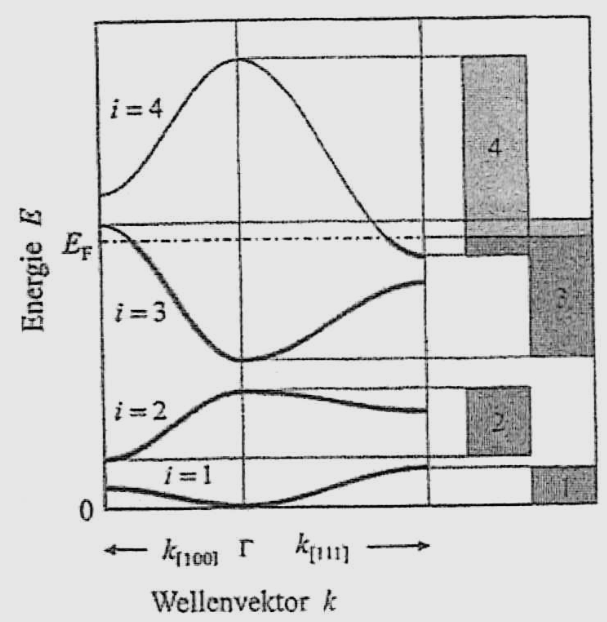
\includegraphics[width = 0.6\linewidth]{figures/vl28/band_richtungsabhaengig.png}
		\caption{Richtungsabhängige Dispersionskurve \cite{Hunklinger}. Die Bänder $i=3$ und $4$ überlappen und es können Elektronen übertreten.
		Ist der Überlapp nur klein, handelt es sich nur um ein Halbmetall.}
	\end{figure}

\paragraph{Beispiel} Stoffe:
	\begin{itemize}
		\item \textbf{Alkalimetalle} \big[z.B. \ce{Na} ($3\mathrm{s}^{1}$), \ce{K} ($4\mathrm{s}^{1}$), \ce{Rb} ($5\mathrm{s}^{1}$)\big] und \textbf{Edelmetalle} \big[z.B. \ce{Cu} ($4\mathrm{s}^{1}$), \ce{Ag}($5\mathrm{s}^{1}$), \ce{Au} ($6\mathrm{s}^{1}$)\big] besitzen ein Valenzlektron pro Atom. Es handelt sich um Metalle.
		
		\item \textbf{Erdalkalimetalle} besitzen zwei Valenzelektronen pro Atom, aber sich überlappende Bänder. Es handelt sich um deshalb um Halbmetalle.

		\item \textbf{Diamant, Silizium und Germanium} besitzen $\mathrm{sp}^{3}$-Hybridorbitale, d.h. pro Atom gibt es vier verfügbare Elektronen. Das Valenzband ist voll und das Leitungsband leer. Es handelt sich um einen Isolator bzw. Halbleiter.
	\end{itemize}

\subsection{Experimentelle Bestimmung von Bandstrukturen}
\subsubsection{Photoemissionsspektroskopie}
	Die Photoemissionsspektroskopie beruht auf Energieniveaus in \autoref{fig:vl28_abbildung_1}.
	\begin{figure}[H]
		\centering
		\def\svgwidth{.433\columnwidth}
		\import{figures/}{vl28_abbildung_1.pdf_tex}
		\caption{Energieschema. 
			Ein Elektron der Energie $E_\mathrm i$ wird mit Licht der Energie $\hbar\omega$ aus dem Festkörper gelöst.
			Dazu überwindet das Elektron die Energie $E_\mathrm B$ von $E_\mathrm i$ zur Fermienergie $E_\mathrm F$, die Austrittsenergie $\varphi_A$, und besitzt die kinetische Energie $E_\mathrm{kin}$ nach dem Austritt.
			Durch Messung der kinetischen Energie können Rückschlüsse auf die Bandenstruktur und die Zustandsdichte gemacht werden.
			}
		\label{fig:vl28_abbildung_1}
	\end{figure}

\paragraph{Lichtquellen}
	Die Photoemissionsspektroskopie kann mit UV-Licht (UPS, \textbf{U}V \textbf{P}hotoemissions-\textbf{S}pektroskopie) oder Röntgenlicht (XPS, \textbf{X}-Ray \textbf{P}hotoemissions-\textbf{S}pektroskopie) durchgeführt werden.
	Bei der UPS werden bspw. \ce{He-}-Gasentladungslampen verwendet, bei der XPS bspw. Röntgenröhren.

	Zur Bestimmung der Bandstruktur verwenden wir den Zusammenhang
	\begin{equation}
		\label{eq:II.8.14}
		\hbar \omega = E_{\text{kin}} + \varphi_{A} + E_{B}.
	\end{equation}
	Für ein festes $\hbar \omega$ erhalten wir ein Spektrum von Elektronen mit verschiedenen $E_{\text{kin}}$.
	Das Spektrum verläuft proportional zur Besetzung $n(E_{\text{kin}})$.
	Wir verwenden
	$$
	E_{B} \text{(variabel)} = \hbar \omega_{\text{fest}} - \varphi_{A} \text{(const)} - E_{\text{kin}} \text{(variabel)}.
	$$ 
	$n(E_{\text{kin}})$ ist somit ein Maß der Zustandsdichte!

	\begin{figure}[H]
		\centering
		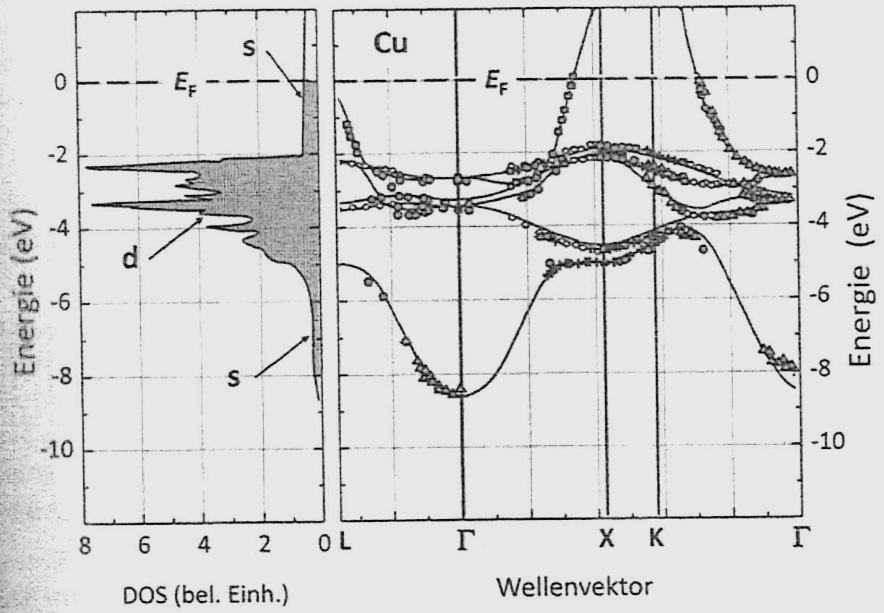
\includegraphics[width = 0.8\linewidth]{figures/vl28/kupfer_zstdichte_baender.png}
		\caption{Zustandsdichte und Bandstruktur von Kupfer \cite{Gross}.}
	\end{figure}
\paragraph{Synchrotron-Strahlungsquellen (UV, XUV, Rö)}\,\\ 
	\begin{figure}[H]
		\centering
		\def\svgwidth{.246\columnwidth}
		\import{figures/}{vl28_abbildung_2.pdf_tex}
		\caption{Schematischer Aufbau eines Synchrotrons. 
			Elektronen werden auf einer Kreisbahn mit Radius $R$ beschleunigt. 
			Bei hohen Geschwindigkeiten bildet das abgestrahlte elektromagnetische Feld des Elektrons eine Keule mit Öffnungswinkel $\theta$.
		}
		\label{fig:vl28_abbildung_2}
	\end{figure}
	Im Synchrotron kann Licht variabler Wellenlänge $\lambda$ bei hoher Intensität erzeugt werden.

	Die Entstehung der Synchrotronstrahlung beruht auf der klassischen Elektrodynamik:
	Diese besagt, dass jede beschleunigte Ladung strahlt.

\paragraph{Beispiel 1: Dipolstrahlung}\,\\
	\begin{minipage}{0.5\linewidth}
		Oszillierende Elektronen erzeugen Dipolstrahlung.
		Im Winkel $\vartheta$ zur Bewegungsachse ist die Intensität der Strahlungsquellen
		$$I\sim\frac{\sin^2\vartheta}{r^2}.$$ 
	\end{minipage}
	\hfill
	\begin{minipage}{0.4\linewidth}
		\begin{figure}[H]
			\centering
			\def\svgwidth{.300\columnwidth}
			\import{figures/}{vl28_abbildung_3.pdf_tex}
			\caption{Elektrisches Feld eines oszillierenden Elektrons.}
			\label{fig:vl28_abbildung_3}
		\end{figure}
	\end{minipage}
	

\paragraph{Beispiel 2: Synchrotron}\,\\[1ex]
	\begin{minipage}{0.5\linewidth}
		Das Elektron bewegt sich im Synchrotron relativistisch mit
		$$v=\SI{0,99987}{\meter\per\second}$$
		bei
		$$E=\SI{1}{\giga\electronvolt}.$$
		Im Laborsystem erscheint sein $\vec E$-Feld als Keule mit Öffnung $\theta$.
		\vspace{1em}
	\end{minipage}
	\hfill
	\begin{minipage}{0.4\linewidth}
		\begin{figure}[H]
			\centering
			\def\svgwidth{.450\columnwidth}
			\import{figures/}{vl28_abbildung_4.pdf_tex}
			\caption{Elektrisches Feld eines Elektrons im Synchrotron.}
			\label{fig:vl28_abbildung_4}
		\end{figure}
	\end{minipage}
	
	Synchrotrons wie das DORIS in Hamburg erzeugen Elektronen mit $E=\SI{3,5}{\giga\electronvolt}$ und $\theta=\SI{0,1}{\milli\radian}$ bei $R=\SI{12.2}{\meter}$.
	
\subsection{Die effektive Massennäherung}
	Wir betrachten Elektronen als Materiewellenpackete mit Wellenvektoren der nächsten Umgebung von $k$:
	$$
	\psi_{n} (\Vec{r},t) = \sum_{k- \frac{\Delta k}{2}}^{k+ \frac{\Delta k}{2}} a(\Vec{k}) u_{\Vec{k}} (\Vec{r}) \exp\left[ i \left( \Vec{k}\Vec{r} - \frac{E_{n}(\Vec{k})}{\hbar }t \right)  \right]
	$$ 

	Dieses Wellenpaket hat die Gruppengeschwindigkeit
	\begin{equation}
		\label{eq:II.8.15}
		\Vec{v}_{g}(\Vec{k}) = \frac{\mathrm{d}\omega(\Vec{k})}{\mathrm{d}\Vec{k}} = \frac{1}{\hbar } \frac{\mathrm{d}E(\Vec{k})}{\mathrm{d}\Vec{k}}.
	\end{equation}

	Der Kristall beeinflusst die Gruppengeschwindigkeit über die Disperionsrelation $E(\Vec{k})$, also über die Bandstruktur. 
	Andererseits ist der Energieübertrag $\mathrm{d}E(\Vec{k})$ in einem Feld
	\begin{equation}
		\label{eq:II.8.16}
		\mathrm{d} E(\Vec{k}) = \Vec{F} \cdot \mathrm{d}\Vec{r} = \Vec{F} \Vec{v}_{\mathrm{g}} \mathrm{d}t.
	\end{equation}
	Mit Gleichung \eqref{eq:II.8.15} folgt die
	\begin{important}
		Bewegungsgleichung für $\vec k$-Vektoren im Impulsraum
		\begin{equation}
			\label{eq:II.8.17}
			\hbar  \frac{\mathrm{d}\Vec{k}}{\mathrm{d}t} = \Vec{F}.
		\end{equation}
	\end{important}
	
	Aus der Zeitableitung von \eqref{eq:II.8.15}
	$$
	\frac{\mathrm{d}\Vec{v}_{\mathrm{g}}}{\mathrm{d}t} = \frac{1}{\hbar } \frac{\mathrm{d}^2 E}{\mathrm{d}k \mathrm{d}t} = \frac{1}{\hbar } \frac{\mathrm{d}^2 E}{\mathrm{d}k^2} \frac{\mathrm{d}k}{\mathrm{d}t}
	$$ 
	folgt mit \eqref{eq:II.8.17}
	$$
	\frac{\mathrm{d} \Vec{v}_{\mathrm{g}}}{\mathrm{d}t} = \left( \frac{1}{\hbar ^2} \frac{\mathrm{d}^2 E}{\mathrm{d}k^2} \right) \Vec{F}.
	$$ 
	Das können wir umformen zur
	\begin{important}
		Bewegungsgleichung in der Form des 2. newtonschen Gesetzes
		\begin{equation}
			\label{eq:II.8.18}
			F = \frac{\hbar ^2}{ \frac{\mathrm{d}^2 E}{\mathrm{d} \Vec{k}^2}} \cdot \frac{\mathrm{d} \Vec{v}_{\mathrm{g}}}{\mathrm{d}t}
		\end{equation}
	\end{important}
	mit der effektiven Masse
	$$
	m^{*} = \frac{\hbar ^2}{ \frac{\mathrm{d}^2 E}{\mathrm{d}\Vec{k}^2}},
	$$ 
	welche in erster Näherung proportional zur Inversen des Krümmungsradius der Bande ist.
